\section{ DISEÑO INTERFAZ DE USUARIO (Pantallas y metodos de clases utilizados)} 
  \subsection{Clase alumno}
  La clase alumno en esta clase esta la informacion necesaria de un alumno para poder participar como usuario de la biblioteca.
	\begin{center}
	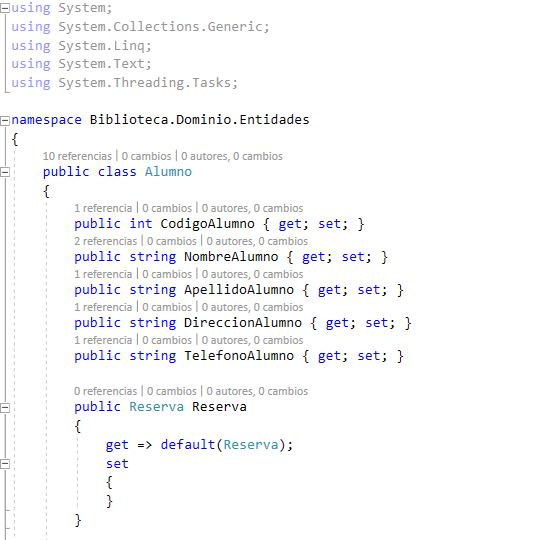
\includegraphics[width=14cm]{./Imagenes/img101} 
	\end{center}

	\begin{center}
	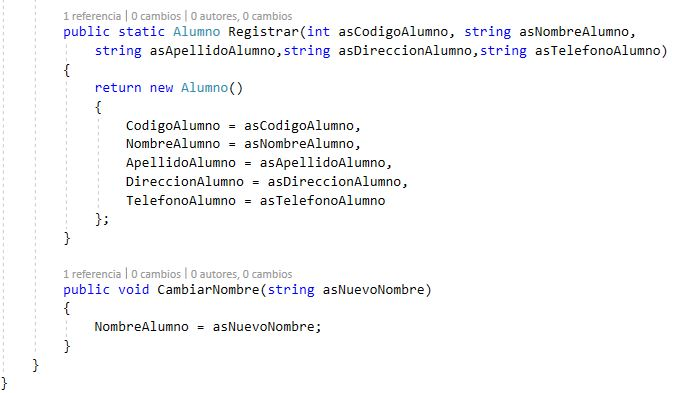
\includegraphics[width=18cm]{./Imagenes/img10} 
	\end{center}
	
 \newpage
 \subsection{Clase libro}
 Dentro de la clase libro encontramos los datos necesarios e infromacion de un libro para poder regitrar en una bilbioteca
 	\begin{center}
	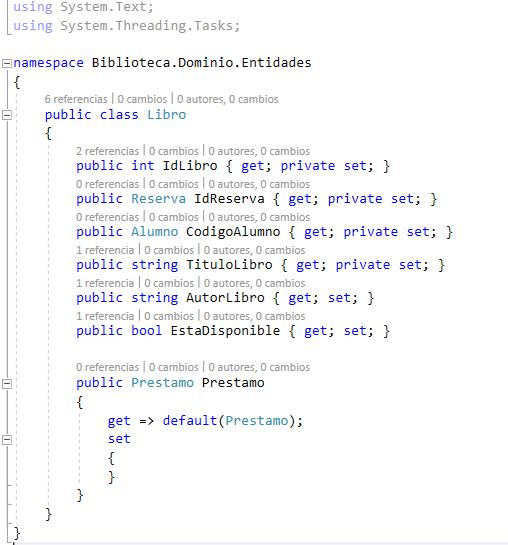
\includegraphics[width=12cm]{./Imagenes/img11libro} 
	\end{center}
	
 \newpage
 \subsection{Clase prestamo}
 Dentro de la clase prestamo encontramos los datos necesarios para realizacion de un prestamos de libro ya sea la fecha la hora y demas datos del alumno que realiza el prestamo y como tambien del bibliotecario.
 	\begin{center}
	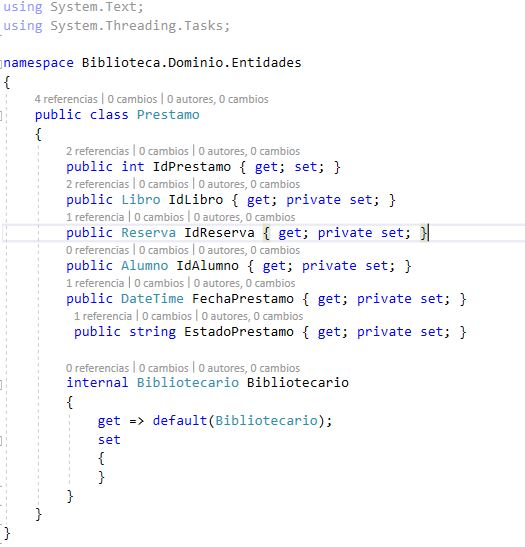
\includegraphics[width=14cm]{./Imagenes/img12prestamo} 
	\end{center}
	
	
 \newpage
 \subsection{Clase Reserva}
 Dentro de la clase resreva encontramos los datos necesarios para realizacion de una reserva de libro como que libro se prestara, su estado entre datos importantes que necesitamos para eralizar la reserva.
 	\begin{center}
	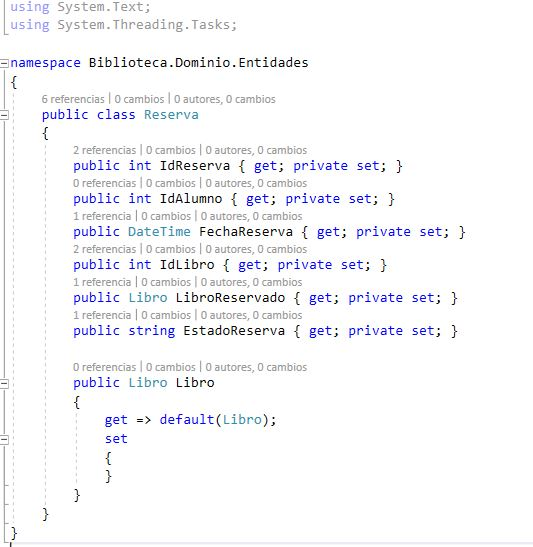
\includegraphics[width=14cm]{./Imagenes/img13reserva} 
	\end{center}
	
 \newpage
 \subsection{Clase Bibliotecario}
 Dentro de la clase  bibliotecario se encuentran los datos del biblbiotecario quien usara el sistema al momento de realizar los prestamos .
 	
